\chapter{Formal Theory}

The Section \ref{sec:description} will outline the key technical ideas using a running example from paper \cite{structured-com-centered-prog}. Sections \ref{sec:flows} and \ref{sec:end-point-calc} outline the global and end-point calculi. Finally, Section \ref{sec:formal-summary} describes the theory of end-point-projection.

\section{Description of communication behaviour}
\label{sec:description}

In this section I will show how small, but complex, business protocol taken from \cite{wscdlprimer} can be accurately and concisely described in two small programming languages developed by the authors of the paper \cite{structured-com-centered-prog}, one based on global message flows and another based on local, end-point behaviours.

\subsection{Simple BSH protocol}

The starting point is simple business protocol for purchasing a good among a buyer, seller and shipper (Simple BSH Protocol). The expected interaction is described as follows:

\begin{figure}
\centering
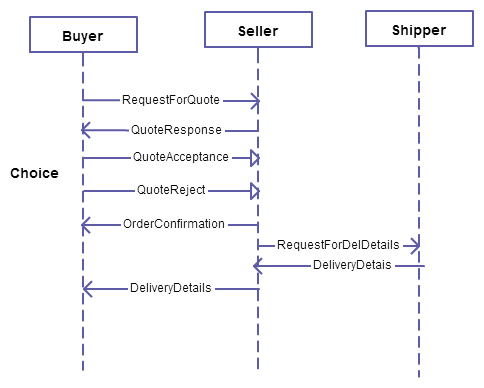
\includegraphics[width=0.8\textwidth]{resources/Simple_bsh.png}
\caption{Simple BSH protocol}
\label{fig:simple-bsh}
\end{figure}

\begin{compactenum}
\item  First, \textit{Buyer} asks \textit{Seller}, through a specified channel, to offer a quote.
\item  Then \textit{Seller} replies with a quote. Buyer then answers with either \textit{QuoteAcceptence} or \textit{QuoteRejection}. If the answer is \textit{QuoteAcceptence}, then Seller sends a confirmation to Buyer, and sends a channel of Buyer to Shipper. Then Shipper sends the delivery details to Buyer, and the protocol terminates. If the answer is \textit{QuoteRejection}, then the interaction terminates.
\end{compactenum}

Figure \label{simple-bsh} presents a UML sequence diagram of this protocol, but many details are left unspecified.

Main assumptions related to both global and local formalisms:
\begin{compactenum}
\item  Each \textit{participant} (Buyer, Seller, Shipper) either communicates through channels or change the content of variables local to it.

\item  All interactions must be dual, e.g. a sender sends a  message and a receiver receives it.

\item  Communication can be either an \textit{in-session communication} which belongs to a session, or \textit{session} \textit{initiation channels} which establishes a session. In a session initiation communication, one or more fresh session channels are declared (belonging to the same session).

\item  A channel can be either a session channel which belongs to a specific session or an session-initiating channel which is used for session-initiation.
\end{compactenum}

Buyer's session-initiating communication in Simple BSH Protocol is described in the global calculus as follows.

\begin{equation}
\text{Buyer} \rightarrow \text{Seller} : \text{quoteCh}(\nu s).I
\label{eq:simple-bsh}
\end{equation}
which says:

Buyer initiates a session with Seller by interacting through a session-initiation channel quoteCh, declaring a fresh in-session channel $s$.

 The symbol ``.'' indicates sequencing as in CSP \cite{com-seq-proc}. A session initiation can specify more than one session channels, as the following example shows.

\begin{equation}
\text{Buyer} \rightarrow \text{Seller} : \text{quoteCh}(\nu \text{B2S}s, \text{S2B}s).I
\end{equation}
which declares two fresh session channels, one from Buyer to Seller and another in the reverse direction.

In local description, the behaviour is split into two, one for Buyer and another for Seller, using the notations from CSP. For example, equation \ref{eq:simple-bsh} becomes:

\begin{equation} 
\text{Buyer}[\text{quoteCh}(s).P1], \text{ Seller}[\overline{\text{quoteCh}}(s).P2]
\label{eq:bsh-split}
\end{equation}

 In \ref{eq:bsh-split},  Buyer[$P$] specifies a buyer's behaviour, while Seller[$P$] specifies a seller's behaviour. The over-lined channel indicates it is used for output.

An in-session communication specifies an operator and, as needed, a message content. For example quote request and response can be written down as follows:

\begin{subequations}
\begin{equation}
\text{Buyer} \rightarrow \text{Seller:B2S}s(\text{QuoteRequest}).I'
\label{eq:quote-request}
\end{equation}
\begin{equation}
\text{Seller} \rightarrow \text{Buyer:S2B}s(\text{QuoteResponse}, 3000, x).I'
\label{eq:quote-response}
\end{equation}
\end{subequations}

For example, the \ref{eq:quote-response} read as follows:

Seller sends a QuoteResponse-message with value 3,000 to Buyer; Buyer upon receipt, assigns the received value, 3,000 to its local variable $x$.

The description of \ref{eq:quote-request} and \ref{eq:quote-response} can be translated to end-point behaviours as follows:

\begin{subequations}
\begin{equation}
\overline{\text{B2S}}s(\text{QuoteRequest}).P1, \text{ B2S}s(\text{QuoteRequest}).P2
\label{eq:end-point-request}
\end{equation}
\begin{equation}
\overline{\text{S2B}}s(\text{QuoteResponse}).P1, \text{ S2B}s(\text{QuoteResponse}).P2
\label{eq:end-point-response}
\end{equation}
\end{subequations}

In various high-level protocols, there is a situation where a sender invokes one of the options offered by a receiver. A method invocation in object-oriented languages is a simplest such example. In a global communication, it is possible to write an in-session communication that involves such a branching behaviour as follows:

\begin{equation}
\begin{split}
\{ \text{Buyer} \rightarrow \text{Seller}&:\text{B2S}s(\text{QuoteAccept}).I1 \} \\ & + \\
\{ \text{Buyer} \rightarrow \text{Seller}&:\text{B2S}s(\text{QuoteReject}).I2 \}
\end{split}
\label{eq:in-session-branching}
\end{equation}
which reads:

``Through an in-session channel B2Ss, Buyer sends one of the two options offered by Seller, QuoteAccept and QuoteReject, and respectively interaction proceeds to $I1$ and $I2$.''

The same interaction can be written down in the local calculus as follows:
\begin{subequations}
\begin{equation}
\text{Buyer's side: } \{ \overline{\text{B2S}s}(\text{QuoteAccept}).P1 \} \oplus \{ \overline{\text{B2S}s}(\text{QuoteReject}).P2 \}
\label{eq:local-calc-buyer}
\end{equation}
\begin{equation}
\text{Seller's side: } \{ \text{B2S}s(\text{QuoteAccept}).Q1 \} + \{ \text{B2S}s(\text{QuoteReject}).Q2 \}
\label{eq:local-calc-seller}
\end{equation}
\end{subequations}

Above $\bigoplus $ indicates that buyer may either behave as $.P1$ or $.P2$, based on its own decision (this is so-called internal sum, whose nondeterminism comes from its internal. Here $+$ indicates this agent may either behave as $.Q1$ or as $.Q2$ depending on what the interacting party communicates through B2Ss (this is so-called external sum, whose nondeterminism comes from the behaviour of an external process). 

The global description of Simple BSH protocol is given in Algorithm \ref{alg:global-description-simple-bsh}.

\begin{algorithm}
\caption{Global description of Simple BSH protocol}
\label{alg:global-description-simple-bsh}
\begin{algorithmic}[1]
    \State Buyer $\rightarrow$ Seller: InitB2S(B2S$s$).
    \State Buyer $\rightarrow$ Seller: B2S$ch$(hQuoteRequest).
    \\
    \State \{ Seller $\rightarrow$ Buyer: B2S$ch$(hQuoteResponse, vquote, xquote).
    \Indstate Buyer $\rightarrow$ Seller: (B2S$ch$ hQuoteAccept).
    \Indstate Seller $\rightarrow$ Buyer: (B2S$ch$ hOrderConfirmation).
    \Indstate Seller $\rightarrow$ Shipper: InitS2H(S2H$s$).
    \Indstate Seller $\rightarrow$ Shipper: S2H$ch$(hRequestDeliveryDetails).
    \Indstate Shipper $\rightarrow$ Seller: S2H$ch$(hDeliveryDetails, vdetails, xdetails).
    \Indstate Seller $\rightarrow$ Buyer: (B2S$ch$ hDeliveryStatus, xdetails, ydetails) .0 \} 
    \State +
    \State \{ Buyer $\rightarrow$ Seller: (B2S$ch$ hQuoteReject) .0 \}
\end{algorithmic}
\end{algorithm}

The local description of Simple BSH protocol is given in Algorithm \ref{alg:local-description-simple-bsh}.

\begin{algorithm}
\caption{Local description of Simple BSH protocol}
\label{alg:local-description-simple-bsh}
\begin{algorithmic}[1]
\State Buyer[ InitB2S(B2S$ch$).
\Indstate B2S$s$(hQuoteRequest).
\Indstate B2S$s$(hQuoteResponce, xquote).
\Indstate[2] \{ B2S$s$(hQuoteAccept).
\Indstate[2] B2S$s$(hOrderConfirmation).
\Indstate[2] B2S$s$(hDeliveryDetails, ydetails) .0 \}
\Indstate[2] +
\Indstate[2] \{ B2S$s$(hQuoteReject) .0 \}]
\\
\State Seller[ InitB2S(B2S$ch$).
\Indstate B2S$s$(hQuoteRequest).
\Indstate B2S$s$(hQuoteResponce, vquote).
\Indstate[2] \{ B2S$s$(hQuoteAccept).
\Indstate[2] B2S$s$(hOrderConfirmation).
\Indstate[2] InitS2H(S2H$s$).
\Indstate[3] S2H$s$(hDeliveryDetails).
\Indstate[3] S2H$s$(hDeliveryDetails, xdetails).
\Indstate[2] B2S$s$(hDeliveryDetails, xdetails) .0 \}
\Indstate[2] +
\Indstate[2] \{ B2S$s$(hQuoteReject $i$) .0 \}]
\\
\State Shipper[ InitS2H(S2H$s$).
\Indstate S2H$s$(hDeliveryDetails).
\Indstate S2H$s$(hDeliveryDetails, vdetails) .0]
\end{algorithmic}
\end{algorithm}


\subsection{Comparison with CDL}

In this section, we briefly outline the relationship between CDL and the global/local calculi used in the previous section. The correspondence/difference are summarized in Table \ref{tab:comparison-cdl}.


\begin{longtable}{|p{0.3\textwidth}|l|l|}
\caption{Comparison analysis of CDL and global/local calculi}\label{tab:comparison-cdl} \\
\hline
\textbf{Feature} & \textbf{CDL} & \textbf{FORMALISM} \\
\hline
\endhead
Session channels & Located at input & No restriction \\
\hline
Session initiation & Implicit & Explicit \\
\hline
{General co-relation} & Yes & No \\ 
\hline 
{Typing} & Informal & Formal \\ 
\hline 
{Type checking} & No & Yes \\ 
\hline 
{Local exception} & None & Yes \\ 
\hline 
{Repetition} & Loop  & recursion \\ 
\hline 
{Sequencing} & Imperative & prefix \\ 
\hline 
{EPP} & Implemented & Proved \\ 
\hline 
{Global variable lookup} & Yes & No \\ 
\hline 
{Global completion} & Yes & No \\ 
\hline 
{Predicate based } & Yes & By adding ``when'' \\ \hline 
\end{longtable}


\section{Global message flows}
\label{sec:flows}

The description of interactions in the global calculus concentrates on a notion of \textit{session}, in which two interacting parties first establish a private connection and do a series of interactions through that private connection, possibly interleaved with other sessions. More concretely, processes first exchange fresh session channels for a newly created session, then use them for interactions belonging to the session (this is equivalent to the more implicit framework where identity tokens in message content are used for signifying a session). This idea has a direct association with a type discipline, where we represent a structured sequence of interactions between two parties as a type. Here type describes an abstract notion of interface of a service, and is inferred by typing rules for each description following its syntactic structure. For example,

\begin{subequations}
\begin{equation}
\text{Buyer} \rightarrow \text{Seller} : s(\text{hRequestQuote}, \text{productName}, xi).
\end{equation}
\begin{equation}
\text{Seller} \rightarrow \text{Buyer} : s(\text{hReplyQuote}, \text{productPrice}, yi).
\end{equation}
\end{subequations}
where, again, a Buyer requests a quote for a product, specifying its name through a session channel $s$. Then through the same channel $s$, a Seller replies with the quote value. This interaction at $s$ can be abstracted by the following session type.

\begin{equation}
s \uparrow \text{RequestQuote}(\text{String}).s \downarrow \text{ReplyQuote}(\text{Int})
\end{equation}

The abstraction is given from a buyer viewpoint. Session type for a seller will be in opposite direction. It is important to note, that there is a natural notion of duality associated with session types.

The formal syntax specification is given in \cite{structured-com-centered-prog}.

\subsection{Reduction}

Computation in the global calculus is represented by a step-by-step transition, each step consisting of:

\begin{compactenum}
\item  Execution of a primitive operation, which can be communication, assignment and conditional.

\item  Effects the execution above has on the local state of an involved participant.
\end{compactenum}

To formalise this idea, we use a configuration which is a pair of a state (a collection of the local states of all participants involved) and an interaction, written $(\sigma, I)$. Formally a state, ranged over by $\sigma, \sigma', \ldots$ is a function from $\text{Var} \times P \rightarrow \text{Val}$, i.e. a variable at each participant is assigned a value in a store. We shall write $\sigma @ A$ to denote the portion of $\sigma$ local to $A$, and $\sigma[ y @ A \rightarrow \nu]$ to denote a new state which is identical with $\sigma$ except that $\sigma'(y, A)$ is equal to $\nu$. The dynamics is then defined in the form:

\begin{equation}
(\sigma, I) \rightarrow (\sigma', I')
\end{equation}
which says $I$ in the configuration $\sigma$ performs one-step computation and becomes $I'$ with new configuration $\sigma'$. The relation $ \rightarrow $ is called reduction relation\footnote{ The term ``reduction'' originally came from  $\lambda$-calculus.}. The following example demonstrates the reduction relation based on recursion:

\begin{equation}
(\sigma, \text{rec}X^B.x@B := 1.X^B) \rightarrow (\sigma[x@B  \mapsto 3], \text{rec}X^B.x@B := 1.X^B)
\end{equation}

All reduction rules are given in \cite{com-centered-basis}.

\subsection{Typing}

As briefly mentioned in previous Section, session types \cite{lang-primitives} are used as the type structures for the global calculus. In advanced web services and business protocols, the structures of interaction in which a service/participant is engaged in may not be restricted to one-way messages or RPC-like request-replies. This is why their type abstraction needs to capture a complex interaction structure of services, leading to the use of session types. The grammar of types presented below.


\begin{equation}
\begin{split}
\Theta & ::= \text{bool} | \text{int} | \dots \\
a & ::= \sum_i s \downarrow op_i(\Theta_i).a_i | \sum_i s \uparrow op_i(\Theta_i).a_i \hspace{1cm} | a_1|a_2|t|\text{rec }t.a|\text{end}
\end{split}
\end{equation}

Above $q, q', \dots$ range over value types, which in the present case only includes atomic data types. $a, a', \dots$ are session types. Note session channels $s, s', \dots$ occur free in session types (this is necessary because of multiple session channels in a single session, cf. \cite{pcalc-control}). In order to be commutative and associative with the identity end, there specified `|'. Recursive types are regarded as regular trees in the standard way \cite{types-and-langs}, \cite{typing-and-subtyping}. The meaning of each construct is given below:

\begin{compactenum}
\item $\sum_i s \downarrow op_i(\Theta_i).a_i$ is a branching input type at $s$, indicating possibilities for receiving any of the operators from $\{op_i\}$ with a value of type $\Theta_i$.

\item $\sum_i s \uparrow op_i(\Theta_i).a_i$, a branching output type at $s$, is the exact dual of the above.

\item  $a_1 | a_2$ is a parallel composition of $a_1$ and $a_2$, abstracting parallel composition of two sessions. We demand session channels in $a_1$ and those in $a_2$ are disjoint.

\item  $t$ is a type variable, while rec $t.a$ is a \textit{recursive type}, where rec $t$ binds free occurrences of $t$ in $a$. A recursive type represents a session with a loop. The main assumption is that each recursion must be guarded, i.e., in rec $t.a$, the type a should be either an input/output type or $n$-ary parallel composition of input/output types.

\item  `end' is the inaction type, indicating termination of a session. `end' is often omitted as we will see in implementation chapter.
\end{compactenum}

Each time a session occurs at a shared service channel, session channels are freshly generated and exchanged. Thus the interface of a service should indicate a vector of session channels to be exchanged, in addition to how they are used. This is represented by abstract session type, or service type, in which concrete instances of session channels in a session type are abstracted, written: 

\begin{equation}
(\tilde{s})\alpha
\end{equation}


The next step is to introduce the notion of duality that was mentioned already in this chapter. So, the co-type, or dual, of $\alpha $ written as $\tilde{\alpha }$ is given as follows,

\begin{equation}
\begin{split}
\overline{\sum_i s \downarrow op_i(\Theta_i).\alpha_i} & = \sum_i s \downarrow op_i(\Theta_i).\overline{\alpha_i} \\
\overline{\text{rec }t.\alpha} & = \text{rec }t.\oveline{\alpha} \\
\overline{t} & = t \\
\overline{\text{end}} & = \text{end}
\end{split}
\end{equation}

\subsection{Examples of session types}

\underbar{Example 1}. Consider the following interaction, assuming `adr' and `prdName' are variables of string type, located at both Buyer and Seller.

\begin{algorithm*}
\begin{algorithmic}[1]
\State Buyer $\rightarrow$ Seller: (s1hQuoteReq, prd, prd).
\State Seller $\rightarrow$ Buyer: (s2hQuoteRep, 100, y).
\State Buyer $\rightarrow$ Seller: (s1hPurchase, adr, adr).0
\end{algorithmic}
\end{algorithm*}

The contract offered by Seller can be described by following session type expression:

\begin{equation*}
s \downarrow \text{QuoteReq}(\text{string}).s2 \uparrow \text{QuoteRep}(\text{int}).s1 \downarrow \text{Purchase}(\text{string}).\text{end}
\end{equation*}

While the interface offered by Buyer can be type-abstracted as follows:

\begin{equation*}
s \uparrow \text{QuoteReq}(\text{string}).s2 \downarrow \text{QuoteRep}(\text{int}).s1 \uparrow \text{Purchase}(\text{string}).\text{end}
\end{equation*}

\underbar{Example 2}. Assume that Example 1 will be preceded by session initiation. Then let assume that session types for Seller and Buyer are $\alpha$ and $\overline{\alpha}$ from Example 1 correspondingly, at the same time the interaction given in Example 1 is $I$. Then:

\begin{equation*}
\text{Buyer} \rightarrow \text{Seller} : \text{ch}(s1,s2).I
\end{equation*}

Then the service type of Seller at channel $sh$ is given as:

\begin{equation*}
(s_1s_2)\alpha \hspace{1cm} (s_1s_2)\overline{\alpha}
\end{equation*}

\underbar{Example 3}. Let Example 1 refine with branching.

\begin{equation*}
\begin{array}{c}
\begin{array}{c}
\text{Buyer} \rightarrow \text{Seller}:s1(\text{QuoteReq, prd, prd}). \\
\text{Seller} \rightarrow \text{Buyer}:s2(\text{QuoteRep}, 100, y).
\end{array}\\
\left(\begin{array}{c} \text{Buyer} \rightarrow \text{Seller}:s1(\text{Purchase, adr, adr}).0 \\ 
+ \text{Buyer} \rightarrow \text{Seller}:s1(\text{NoDanke}).0
\end{array}\right)
\end{array}
\end{equation*}

This can be abstracted, from the viewpoint of Seller:

\begin{equation*}
\begin{array}{c}
s1 \downarrow \text{QuoteReq}(\text{string}).s2 \uparrow \text{QuoteRep}(\text{int}).(s1 \downarrow \text{Purchase}(\text{string}).end + \\ + s1) \downarrow \text{NoThanks}().\text{end}
\end{array}
\end{equation*}

The typing rules are given in paper \cite{com-centered-basis}.

\section{End-point calculus}
\label{sec:end-point-calc}

The end-point calculus, an applied variant of the p-calculus \cite{poly-p-calc}, specifies local behaviours of end-points and their composition. For example consider the following term in the global calculus (cf. Example 1):

\begin{equation*}
\text{Buyer} \rightarrow \text{Seller} : s(\text{QuoteAccept}, 100, x, ., 0)
\end{equation*}

This global description says that Buyer sends a `QuoteAccept' message with value 100 to Seller, that Seller receives it, and that Seller saves this value in its local variable $x$. The end-point calculus describes the same situation as combination of local behaviour, located at each end-point. First there is Buyer's behaviour:

\begin{equation*}
\text{Buyer}[\overline{s} \triangleright \text{QuoteAccept}(100).\textbf{0}]\sigma_B
\end{equation*}
where $\sigma_B$ is Buyer's local state. Similarly we have Seller's local behaviour:

\begin{equation*}
\text{Seller}[s \triangleright \text{QuoteAccept}(x).\textbf{0}]\sigma_S
\end{equation*}
where $\sigma_S$ is Seller's local state. Interaction takes place when are concurrently composed, as follows.

\begin{equation*}
\text{Seller}[s \triangleright \text{QuoteAccept}(x).\textbf{0}]\sigma_S | \text{Buyer}[\overline{s} \triangleright \text{QuoteAccept}(100).\textbf{0}]\sigma_B
\end{equation*}
Let this term be written $T$. Then the communication event is represented using the following one-step reduction:

\begin{equation*}
T \rightarrow \text{Seller}[\textbf{0}]_{\sigma_s[x \mapsto 10]}|\text{Buyer}[\textbf{0}]_{\sigma_B}
\end{equation*}
where the seller is updated as a result of communication. Communication in local calculus is organized in the unit of session. To avoid a situation when local behaviours of participants does not correspond to their global specification, the type discipline is used. For example, the expression above can be abstracted as follows:

\begin{equation*}
s@\text{Buyer}:s\uparrow\text{QuoteAccept}(\text{int}).\text{end}
\end{equation*}
while that of Seller is abstracted as:

\begin{equation*}
s@\text{Seller}:s\downarrow\text{QuoteAccept}(\text{int}).\text{end}
\end{equation*}
Since two signatures are clearly compatible, we conclude the composition is well-typed.

\subsection{Examples}

Simple BSH protocol may have the following end-point version:

\begin{equation*}
\begin{array}{c}
\text{Buyer}[\text{B2S}Chs].s \triangleright \text{RequestForQuote}.s \triangleleft \text{QuoteResponse}(\text{xquote}). \\
s \triangleright (\text{QuoteReject} + \text{QuoteAccept}.s \triangleleft \text{OrderConfirmation}.s \triangleright \text{DeliveryDetails})]a | \\
\text{Seller}[\text{B2S}Ch(s).s \triangleleft \text{RequesForQuote.s} \triangleright \text{QuoteResonse}h \nu \text{quote} i.s \triangleleft \\
 (\text{QuoteReject} + \text{QuoteAccept}.s \triangleright \text{OrderConfirmation}.\text{S2H}hChhs'i.s' \triangleright \\
\text{RequestDelDetailsBuyer}i.s \triangleright \text{DeliveryDetails}(xDD) \\
s \triangleleft \text{DeliveryDetails}]b|\\
\text{Shipper}[\text{S2S}hCh(s').s' \triangleleft \text{RequestDelDetails}(x\text{Cilent}).s \triangleright \text{DeliveryDetails}(DD)]g
)
\end{array}
\end{equation*}

\section{Summary}
\label{sec:formal-summary}

In preceding sections, I have presented example specifications both as a global view in the global calculus and as a local view written in the end-point calculus. In doing so, a global description was always introduced first, and from that the corresponding end-point processes were being recovered. From an engineering viewpoint, these two steps --- start from a global description, then extract out of it a local description for each end-point --- offer an effective methods for designing and coding communication-centric programs. ``It is often simply a pain to design, implement and validate an application that involves complex interactions among processes and which together work correctly, if we are to solely rely on descriptions of local behaviours.'' This is why such tools as message sequence charts and sequence diagrams have been used as a primary way to design communication behaviour. In fact, the primary concern of the design/requirement of communication behaviour of an application would in general be how global information exchange among processes will take place and how these interactions lead to desired effects: the local behaviour of individual components only matter to realize this global scenario. Thus, in designing and implementing communication-centric software, one may as well start from a global description of expected behaviour, then translate it into local descriptions. 

Translating a global description to its end-point counterpart, the process called end-point projection, can however be tricky, because it can be easily produced a global description which does not correspond to any reasonable local counterpart. In other words, if you do not follow good principles, the global description does not in fact describe realizable interaction (not well-formed).


